
%----------------------------------------------------------------------------------------
%   PACKAGES AND DOCUMENT CONFIGURATIONS
%----------------------------------------------------------------------------------------

\documentclass{article}

\usepackage{siunitx} % Provides the \SI{}{} and \si{} command for typesetting SI units
\usepackage{graphicx} % Required for the inclusion of images
\usepackage{natbib} % Required to change bibliography style to APA
\usepackage{amsmath} % Required for some math elements 
\usepackage{csvsimple}
\usepackage{caption}
\usepackage{multicol}
\usepackage{rotating}

\setlength\parindent{0pt} % Removes all indentation from paragraphs

\renewcommand{\labelenumi}{\alph{enumi}.} % Make numbering in the enumerate environment by letter rather than number (e.g. section 6)

%\usepackage{times} % Uncomment to use the Times New Roman font

%----------------------------------------------------------------------------------------
%   DOCUMENT INFORMATION
%----------------------------------------------------------------------------------------

\title{Projectile Motion and Conservation of energy \\ PHYS 1493} % Title

\author{Jeffrey Wan jw3468} % Author name

\date{\today} % Date for the report

\begin{document}

\maketitle % Insert the title, author and date

\begin{center}
\begin{tabular}{l r}
Date Performed: & Septemeber 25, 2017 \\ % Date the experiment was performed
Partners: & Pranav Shrestha ps2958\\ % Partner names
& Greyson Barrera gmb2167\\
\end{tabular}
\end{center}

% If you wish to include an abstract, uncomment the lines below
% \begin{abstract}
% Abstract text
% \end{abstract}

%----------------------------------------------------------------------------------------
%   Objective
%----------------------------------------------------------------------------------------

\section{Introduction}

In this experiment, we test our ability to predict the motion of a small projectile using simple equations. We will carry out a series of trials and perform statistical analysis. We will then compare our data to expected values derived using equations \eqref{eq:1}, \eqref{eq:2}, and \eqref{eq:3}.

\hspace{1cm}

\textbf{Work by Friction}
\begin{equation}\label{eq:1} 
    W_{f} = mg(h_{1}\ensuremath{'} - h_{2}\ensuremath{'})
\end{equation}

\textbf{Initial Velocity}
\begin{equation}\label{eq:2}
    v_{0} = \sqrt{\frac{10}{7m}(mg(h_{1}-h_{2})-W_{f})}
\end{equation}

\textbf{Projectile Motion}
\begin{equation}\label{eq:3} 
    V_{x}(t) = V_{0} cos(\theta), \quad V_{y}(t) = V_{0} sin(\theta) - gt
\end{equation}


%----------------------------------------------------------------------------------------
%   Method
%----------------------------------------------------------------------------------------
\section{Method}
\begin{enumerate}

    \item Estimate the work done by friction 
        \begin{enumerate}
            \item Adjust the ramp angle adjustment screw such that when the sphere is released at the release point, the sphere makes it just to the edge of the ramp before reversing direction.
            \item Record measurements $h_{1}\ensuremath{'}$, and $h_{1}\ensuremath{'}$.
            \item Use equation \eqref{eq:1} to derive work done by friction $W_{f}$. Note that the mass of the sphere is not necessary. Calculating $\frac{W_{f}}{m}$ will suffice since $m$ will be canceled out in equation \eqref{eq:2}.
        \end{enumerate}

    \item Conduct Trials
        \begin{enumerate}
            \item Adjust the ramp angle adjustment screw such that: \\
                \begin{equation} h_{1} - h_{2} > 2(h_{1}\ensuremath{'} - h_{2}\ensuremath{'}) \end{equation}
            \item Use the new measurements of the ramp $h_{1}, h_{2}, h_{3}, D, L$ and the equations \eqref{eq:1}, \eqref{eq:2}, and \eqref{eq:3}, to predict where the sphere will land. 
            \item Release the sphere from the release point and confirm if the prediction is accurate.
            \item Place a sheet of white paper on the floor where the sphere is predicted to land.
            \item Place a sheet of carbon paper on top of the white paper. Tape both down.
            \item Draw crosshairs on the sheet through the point where the sphere is predicted to land.
            \item Release the sphere 20 times and record the results.

        \end{enumerate}

    \item Repeat the procedure for a different set of measurements, $h_{1}, h_{2}, h_{3}, D, L$ and a different sphere.
\end{enumerate}
 
%----------------------------------------------------------------------------------------
%   Data 
%----------------------------------------------------------------------------------------
\clearpage
\section{Data}

\begin{multicols}{2} \begin{center} \begin{small}
    \begin{tabular} {|l|l|} 
        \hline
        \bfseries x(cm) & \bfseries z(cm)
        \csvreader[head to column names]{m1.csv}{}
        {\\\hline\csvcoli&\csvcolii}
        \\\hline
    \end{tabular}
    \captionof{table}{Metal, Trial 1}

    \hspace{1cm}

    \begin{tabular} {|l|l|} 
        \hline
        \bfseries x(cm) & \bfseries z(cm)
        \csvreader[head to column names]{p1.csv}{}
        {\\\hline\csvcoli&\csvcolii}
        \\\hline
    \end{tabular}
    \captionof{table}{Plastic, Trial 1}


    \begin{tabular} {|l|l|} 
        \hline
        \bfseries x(cm) & \bfseries z(cm)
        \csvreader[head to column names]{m2.csv}{}
        {\\\hline\csvcoli&\csvcolii}
        \\\hline
    \end{tabular}
    \captionof{table}{Metal, Trial 2}

    \hspace{1cm}

    \begin{tabular} {|l|l|} 
        \hline
        \bfseries x(cm) & \bfseries z(cm)
        \csvreader[head to column names]{p2.csv}{}
        {\\\hline\csvcoli&\csvcolii}
        \\\hline
    \end{tabular}
    \captionof{table}{Plastic, Trial 2}
\end{small} \end{center} \end{multicols}

\begin{center} \begin{footnotesize}
    \begin{tabular} {|l|l|l|l|l|l|l|l|l|} 
        \hline
        Sphere & Trial & $h_{1}\ensuremath{'}$ (cm)& $h_{2}\ensuremath{'}$ (cm)&$h_{1}$ (cm)& $h_{2}$ (cm)& D (cm)& L (cm)&$h_{3}$(cm)
        \csvreader[head to column names]{meta.csv}{}
        {\\\hline\csvcoli&\csvcolii&\csvcoliii&\csvcoliv&\csvcolv&\csvcolvi&\csvcolvii&\csvcolviii&\csvcolix}
        \\\hline
    \end{tabular}
    \captionof{table}{Measurements of each trial}
\end{footnotesize}\end{center}


%----------------------------------------------------------------------------------------
%   Data Analysis
%----------------------------------------------------------------------------------------
\clearpage
\section{Data Analysis}
We calculate the mean and the errors as described by equations \eqref{eq:5}, \eqref{eq:6}, and \eqref{eq:7}.
\hspace{1cm}
\hspace{1cm}

\textbf{Mean}
\begin{equation} \label{eq:5}
    \bar{x} = \sum_{i=1}^{N} x_{i}
\end{equation}

\textbf{Sample Standard Deviation}
\begin{equation} \label{eq:6}
    s = \sqrt{\frac{\sum (x_{i} - \bar{x})^2}{N-1}}
\end{equation}

\textbf{Standard Error}
\begin{equation} \label{eq:7}
    \sigma_{x} = \frac{s}{\sqrt{N}}
\end{equation}

\hspace{1cm}

\begin{center}
\begin{tabular} {|l|l|l|l|} 
    \hline
    \bfseries Sphere & \bfseries Trial & \bfseries $\bar{x}\pm\sigma_{x}$ (cm)& \bfseries $\bar{z}\pm\sigma_{z}$ (cm)\\\hline
    Metal&1&$2.637\pm0.062$&$0.003\pm0.054$\\\hline
    Plastic&1&$2.67\pm0.11$&$2.28\pm0.15$\\\hline
    Metal&2&$2.030\pm0.060$&$2.710\pm0.052$\\\hline
    Plastic&2&$-1.98\pm0.13$&$-2.01\pm0.11$\\\hline
\end{tabular}
\captionof{table}{Observed Means and their uncertainties}
\end{center}

\begin{sidewaysfigure}[h]
\begin{center}
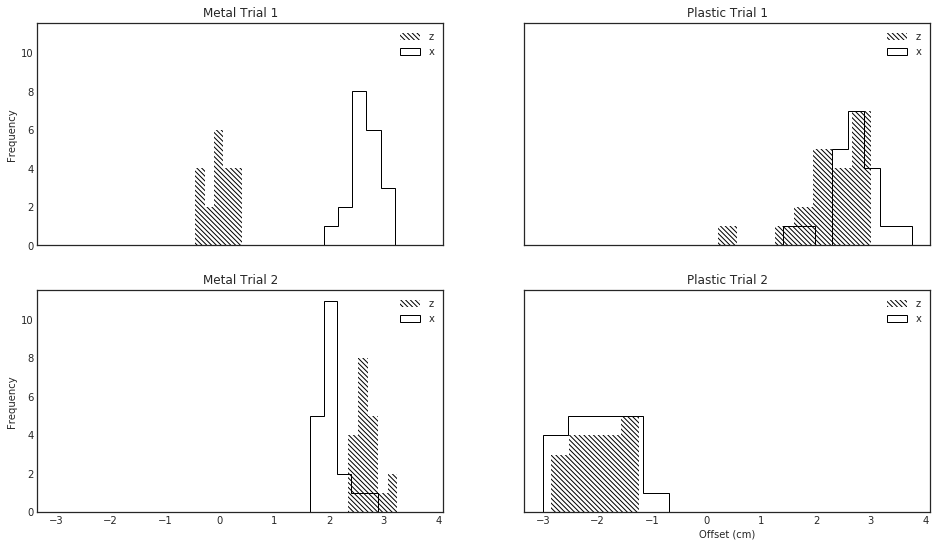
\includegraphics[width=1\textwidth]{hist.png} % Include the image placeholder.png
    \caption{Difference between actual and expected positions}
    \label{fig:hist}
\end{center}
\end{sidewaysfigure}

In figure \ref{fig:hist}, even though all the distributions are roughly bell-shaped, only the first trial of the metal sphere has a distribution that centered around the expected value. In the remaining trials, the overall shift in the points is evident of systematic errors. There are many factors that could have caused this shift. Two possible factors include the presence of wind in the room toward one direction, and a error in the direction of the release ramp during setup. Furthermore, in each trial, the degree of spread in the x and z directions are very similar. However, the trials for the metal sphere had significantly smaller spread than those of the plastic balls. This could be attributed to the fact that the metal balls have more mass, and thus their trajectories are less prone being affected by the random changes in the wind. Additionally, the plastic is not a conductor, which means that it is able to hold a charge. The plastic's trajectory may be affected by electromagnetic forces. Altercations to reduce spread include performing the experiment in a vacuum, getting rid of static electricity, using denser spheres such as those made from lead. 

If instead, a hollow plastic sphere was used for the experiment, its moment of inertia would increase and its mass decreases. This would cause $v_{0}$ to decrease. Thus, mean distance would decrease, and spread increases.




%----------------------------------------------------------------------------------------
%   Conclusions
%----------------------------------------------------------------------------------------
\clearpage
\section{Conclusions}

The accepted value (periodic table) is \SI{24.3}{\gram\per\mole} \cite{Smith:2012qr}. The percentage discrepancy between the accepted value and the result obtained here is 1.3\%. Because only a single measurement was made, it is not possible to calculate an estimated standard deviation.

The most obvious source of experimental uncertainty is the limited precision of the balance. Other potential sources of experimental uncertainty are: the reaction might not be complete; if not enough time was allowed for total oxidation, less than complete oxidation of the magnesium might have, in part, reacted with nitrogen in the air (incorrect reaction); the magnesium oxide might have absorbed water from the air, and thus weigh ``too much." Because the result obtained is close to the accepted value it is possible that some of these experimental uncertainties have fortuitously cancelled one another.
j
 %----------------------------------------------------------------------------------------
 %   BIBLIOGRAPHY
 %----------------------------------------------------------------------------------------

 \bibliographystyle{apalike}

 \bibliography{sample}

 %----------------------------------------------------------------------------------------
 \end{document}
